\documentclass[a4paper, 11pt]{article}
\usepackage[left=3cm, right=3cm, top=2.54cm, bottom=2.54cm]{geometry}
\usepackage{graphicx}
\usepackage{kotex}
\usepackage[onehalfspacing]{setspace}
\renewcommand{\contentsname}{차  례}
\usepackage{indentfirst}
\usepackage[bookmarks=true,pdfborder={0 0 0}]{hyperref}

\title{전자 피아노}

\begin{document}

\begin{titlepage}
\vspace{4cm}
\begin{center}
{\huge \textbf{2019 임베디드 시스템 설계 및 실험\\ 프로젝트 제안서}}\\[2cm]
{\Huge \textbf{전자피아노}}\\[2cm]
{\Large 목요일(004분반) 제3조 }\\[3cm]
\tableofcontents
\end{center}
\end{titlepage}

\section{개요와 현황}

\subsection{개요}
  이 프로젝트는 임베디드 시스템을 이용하여 전자 악기를 구현하는 프로젝트이다. 전자악기는 보통 전자적 장치에 사운드 폰트를 저장하여 실제 악기의 메커니즘을 적용한다. 가장 고전적인 전자 피아노는 MIDI 신디사이저를 물리적인 건반에 전자회로로 연결하여 MIDI 신호를 주고받는다. 이 때, MIDI 신디사이저에서는 각 미디 신호에 따른 사운드 폰트를 저장하고 있고, 미리 신디사이저에 설정한 사운드폰트를 출력하는 것으로 악기를 연주하는 것이다.
     
\subsection{현재 전자피아노의 현황}

현재 전자 피아노 시장은 판매대수를 기준으로 연 10\% 이상 성장 중이다. 전자 피아노는 일반 어쿠스틱 피아노에 비해 매우 저렴한 가격과 뛰어난 공간성을 가지고 있고, 층간 소음문제와 같은 문제에서 비교적 자유롭다. 이러한 특징들로 1인 가구에게 특히 인기를 끌고 있다. 
전자 피아노 기술의 핵심은 “얼마나 실제 피아노와 같은 소리를 낼 수 있는가” 이다. 압력을 여러 단계로 Sampling 하여 소리의 세기를 세분화 하는 기술이 기본적인데, 얼마나 민감한 센서를 이용하여 어떻게 압력을 Sampling 할 것인지가 중요하다. 최대한 피아노의 연주 기법에 따른 소리를 담아 낼 수 있도록 하는 것이 핵심 기술력이다. 

\section{해결과제 설정}
\subsection{과제개요}
이 프로젝트를 완수하기 위하여 해결하여야할 최소의 과제는 다음과 같다. 
\begin{itemize}
\item 임베디드 시스템에서 오디오를 재생하는 기능을 구현하여야 한다.
\item 압력을 감지하는 장치를 임베디드 시스템에 연결하여 압력 센서에 일정한 압력이 들어왔을 때, 배정된 사운드 폰트를 재생하여야 한다.
\end{itemize}

\subsection{하드웨어적 요구사항}
  이 과제를 수행하기 위한 세부 하드웨어 요구사항은 다음과 같다.
\begin{enumerate}
\item 압력센서는 사용자의 압력에 비례한 값을 주어야 한다. 
\item LCD는 출력된 화면을 보고 사용자가 파일을 선택할 수 있어야 하므로 터치 기능을 지원하여야 한다. 
\item 임베디드 시스템의 기본 제어 장치는 Cortex-M3를 채용한 STM32F107VC를 기반으로 한 실습 보드로 한다.
\item 건반은 압력센서와 물리적인 방법으로 연결되어야 하며, 90\% 이상의 인식율을 지녀야 한다. 
\item DSTREAM과 연결되지 않은 상태에서도 기능이 작동하여야 한다. 
\item JoyStick과 UserButton에 대하여 인터럽트 방식 입력을 지원하여야 한다.
\item 오디오 코덱은 8Khz 이상의 스테레오 음질을 보장하여야 한다. 
\item 기본 제어장치의 3.5$\phi$ 잭에 음성 출력 장치를 연결하면, 그 연결된 장치에서 소리가 출력되어야 한다.
 
\begin{figure}[h!]
\centering
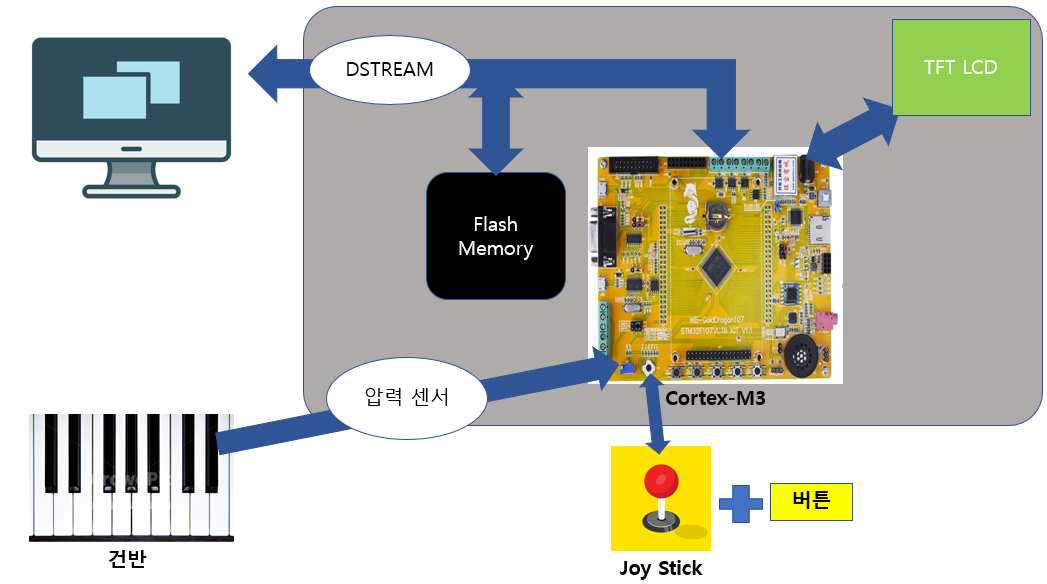
\includegraphics[width=\linewidth]{./Figure/HW.png}
\caption{HW 구성도}
\label{Fig:Fig0}
\end{figure} 

\end{enumerate}
\subsection{소프트웨어적 요구사항}
  이 과제에서 구현하여야 할 소프트웨어적 요구사항은 다음과 같다. 
\begin{enumerate}
\item 제어 보드에 전원이 인가되었을 때, 시스템은 IDLE상태를 유지한다. 
\item IDLE 상태에서는 OTG-USB로 연결된 플래시 메모리에 있는 파일 목록을 출력하여야 한다. 
\item IDLE 상태에 연주버튼을 누를경우 연주상태가 시작된다. 
\item 연주상태에서는 다음의 상태를 말한다. 
\begin{enumerate}
\item 연주상태에서는 타이머를 통해 시간을 기억하며 건반을 누를 때, 건반에 연결된 압력센서로부터 압력에 따른 값을 입력받는다.
\item 압력에 따른 값에 비례하여 해당 음계의 소리를 출력하며, 메모리에 (세기, 옥타브, 음계, 누른시간, 뗀 시간)의 구조체로 기록한다. 
\item 연주상태에서 연주버튼을 한번 더 누를 경우에는 연주상태를 종료하고 IDLE 상태로 복귀한다. 이 때, 기록된 구조체들을 OTG-USB에 파일로 저장한다.   
\item 조이스틱을 활용하면 옥타브를 올리거나 내릴 수 있다. 
\end{enumerate}
\item IDLE 상태에서 LCD 터치패널을 통해 파일을 선택하여 악보 표시상태로 변경한다. 
\begin{enumerate}
\item 악보상태에서는 선택된 바이너리 파일을 읽어서 각 구조체의 데이터에 맞추어 소리를 출력한다.
\item LCD 터치패널을 통하여 악보상태를 종료할 수 있다. 또한, 파일의 마지막을 연주한 때는 악보상태가 종료된다.  
\end{enumerate}
\end{enumerate}

\begin{figure}[h!]
\centering
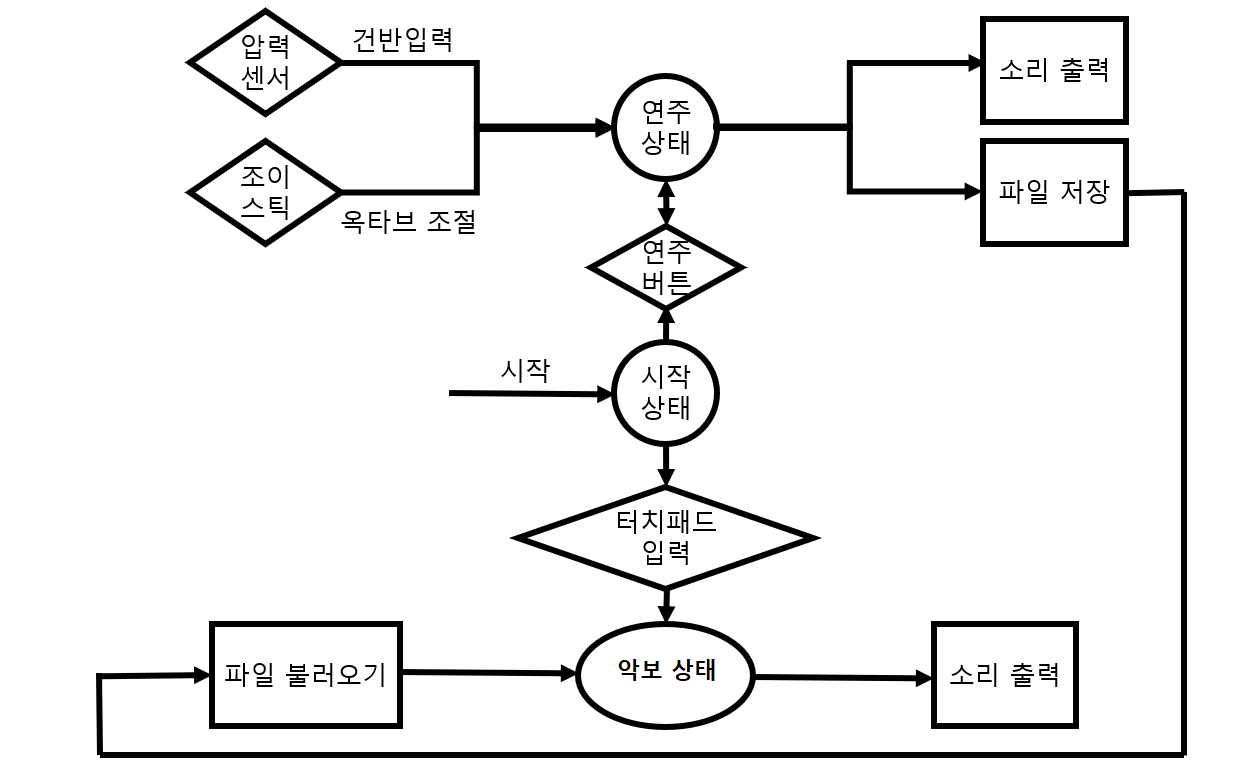
\includegraphics[width=\linewidth]{./Figure/SW.png}
\caption{소프트웨어 흐름도(Flowchart)}
\label{Fig:Fig1}
\end{figure}

\newpage
\section*{Appendix. 필요 센서 명세}
\addcontentsline{toc}{section}{\protect\numberline{A }필요 센서 명세}
{\large{\textbf{1. 압력센서 브릿지}}}

\begin{figure}[h!]
\centering
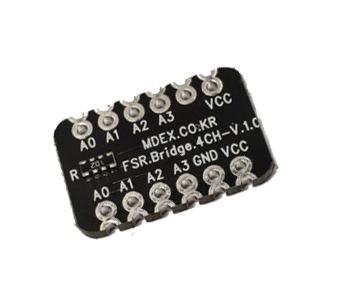
\includegraphics[scale=0.7]{./Figure/CF1.png}
\end{figure}

\begin{itemize}
\item 수량 : 3EA
\item 제품명 : 압력센서 브릿지-4채널
\item 제조사 : 마블덱스
\item URL : \url{http://www.devicemart.co.kr/goods/view?no=1385810}
\end{itemize}

\textbf{특징}

\begin{itemize}
 \item 가로 : 18.7mm 
 \item 세로 : 12.0mm 
 \item 저항 10k$\mathrm{\Omega}$
 \item 4개의 압력센서를 묶어서 풀다운 저항 따로 설정할 필요없이 사용가능
\end{itemize}

\noindent {\large \textbf{2. 압력센서}}

\begin{figure}[h!]
\centering
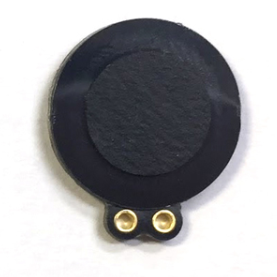
\includegraphics[scale=0.7]{./Figure/CF3.png}
\end{figure}

\begin{itemize}
\item 수량 : 12EA
\item 제품명 : 압력센서 FSR, RA12P
\item 제조사 : 마블덱스
\item URL : \url{http://www.devicemart.co.kr/goods/view?no=1327467}
\end{itemize}

\textbf{특징}
 
\begin{itemize}
\item 길이 : 14.15mm 
\item 폭 : 12mm
\item 두께 : 1.55mm 
\item 센싱압력범위 : 5g $\sim$ 4kg
\item 10k$\mathrm{\Omega}$ 저항 사용시 0 $\sim$ 5V 전압얻을수있음
\end{itemize}


\noindent {\large \textbf{3. TFT-LCD (8주차 실험 예정 준비물) }}

\begin{figure}[h!]
\centering
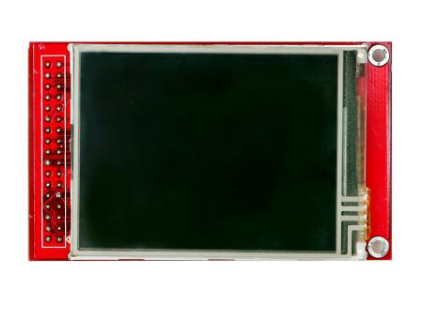
\includegraphics[scale=0.7]{./Figure/CF4.png}
\end{figure}

\begin{itemize}
\item 크기 : 3.2" 
\item 컬러 가능, 터치 지원.
\end{itemize}


\noindent {\large \textbf{4. 하드웨어 코덱}}
\begin{figure}[h!]
\centering
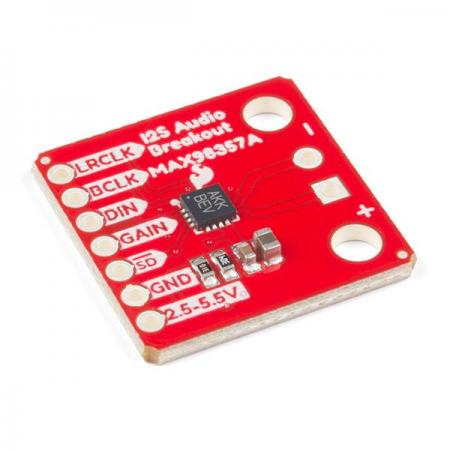
\includegraphics[scale=0.6]{./Figure/CF5.jpg}
\end{figure}


\begin{itemize}
\item 수량 : 1EA
\item 제품명 : MAX98357A
\item 제조사 : SparkFun
\item 4옴 스피커를 연결할 수 있는 장치
\item URL : \url{http://www.devicemart.co.kr/goods/view?no=10824349}
\end{itemize}

\noindent {\large \textbf{5. 4옴 스피커}}
\begin{figure}[h!]
\centering
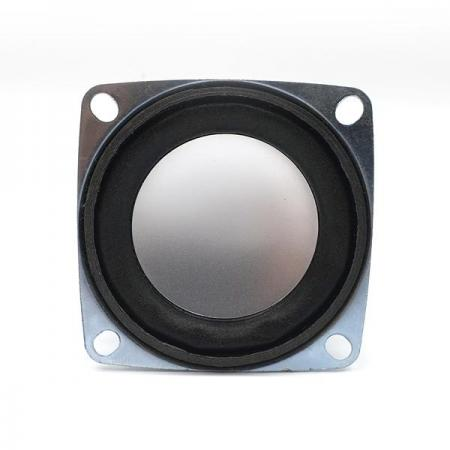
\includegraphics[scale=0.6]{./Figure/CF6.jpg}
\end{figure}


\begin{itemize}
\item 수량 : 1EA
\item 제품명 : SY-SPK059
\item 4옴 임피던스 스피커
\item URL : \url{http://www.devicemart.co.kr/goods/view?no=12236769}
\end{itemize}


\end{document}